\documentclass[12pt, letterpaper]{article}
\usepackage[colorlinks]{hyperref}
\usepackage[utf8]{inputenc}
\usepackage{graphicx}
\usepackage[font=small,skip=-1pt]{caption}
\usepackage{subcaption}
\usepackage{amsmath}
\usepackage{placeins}
\usepackage{listings}
\usepackage{color}

\definecolor{dkgreen}{rgb}{0,0.6,0}
\definecolor{gray}{rgb}{0.5,0.5,0.5}
\definecolor{mauve}{rgb}{0.58,0,0.82}

\lstset{frame=tb,
	language=Java,
	aboveskip=3mm,
	belowskip=3mm,
	showstringspaces=false,
	columns=flexible,
	basicstyle={\small\ttfamily},
	numbers=none,
	numberstyle=\tiny\color{gray},
	keywordstyle=\color{blue},
	commentstyle=\color{dkgreen},
	stringstyle=\color{mauve},
	breaklines=true,
	breakatwhitespace=true,
	tabsize=3
}

\graphicspath{ {./plots/} }

\title{Analysis Report on Inspecting MQTT}
\author{Liyao Tang - u6142160}
\date{ \today}

\begin{document}
\begin{titlepage}
	\maketitle
\end{titlepage}

\section{Analysis on Handshakes under Different QoS}

Figure \ref{fig:handshake_snap_shot} shows the required screenshots. QoS defines the handshake of the sending and receiving of one message between the sender and receiver, which both can be either broker or devices. For each QoS level, an explanation of its handshake are given as follow.
\begin{enumerate}

	\item QoS = 0
	
	The application message is delivered according to the best efforts of the underlying TCP/IP network and sender would discard the application message once sent out. 
	
	Hence, the application message will arrive at receiver at most once.
	
	\item QoS = 1
	
	After application message sent, sender waits for an acknowledgement (PUBACK or Publish Ack) to make sure the application message is received. To match PUBACK with corresponding application message, each application message at this QoS level has an ID. After PUBACK received, application message can be safely discarded.
	
	After a predefined time without returning PUBACK for the application message, sender will re-send application message with its DUP flag set, meaning this is duplicate. 
	
	Hence, the application message will arrive at receiver at least once.
	
	\item QoS = 2
	
	After application message sent, sender waits for an acknowledgement (PUBREC or Publish Received) to ensure application message is received and then responds with a further acknowledgement (PUBREL or Publish Release) to acknowledge that it knows application message is received. Afterwards, sender still needs to wait for one more acknowledgement (PUBCOMP or Publish Complete) from receiver so that sender is sure that receiver has received the PUBREL. Finally, the application message can be safely discarded.
	
	After a predefined time without the expecting message, the protocol (either sender or receiver) will retry from the last unacknowledged message.
	
	Hence, the application message will arrive at receiver exactly once.
	
\end{enumerate}

As listed above, those assisting messages that is not compulsory for application to meet its specification can transmit on QoS level 0; whereas those key messages, which may results in deviation from the specification if not received, should transmit under QoS level 1; while some important messages whose not only payload but also occurrence matter should transmit under QoS level 2 because duplicate messages are not allowed under this circumstance.

\begin{figure}
	\centering
	\begin{subfigure}[t]{0.77\textwidth}
		\centering
		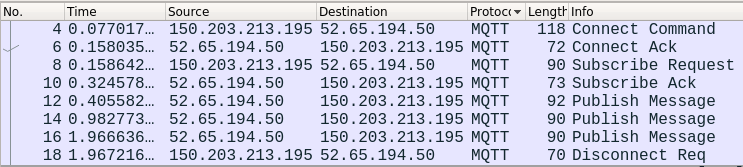
\includegraphics[width=\textwidth]{wire_shark/handshake-q0}
		\caption{QoS = 0}
	\end{subfigure}
	
	\begin{subfigure}[t]{0.77\textwidth}
		\centering
		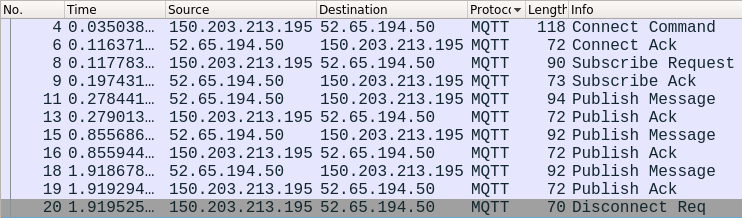
\includegraphics[width=\textwidth]{wire_shark/handshake-q1}
		\caption{QoS = 1}
	\end{subfigure}
	
	\begin{subfigure}[t]{0.77\textwidth}
		\centering
		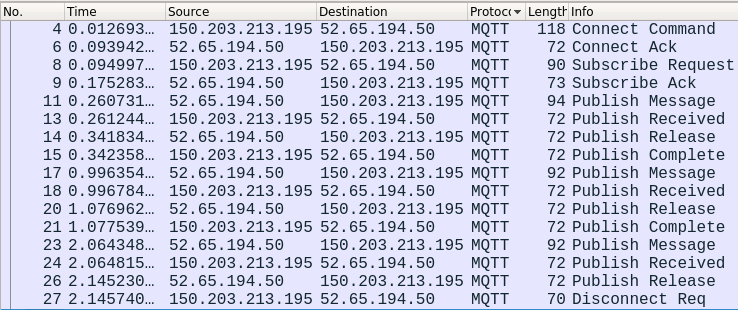
\includegraphics[width=\textwidth]{wire_shark/handshake-q2}
		\caption{QoS = 2}
	\end{subfigure}

	\caption{Figures of MQTT handshake under different QoS. The client disconnects the broker after receives three messages.}
	\label{fig:handshake_snap_shot}
\end{figure}

\section{Statistical Analysis for Each QoS Level}

\subsection{Collecting Statistics}

\subsubsection{Code Structure and Explanation}

The code is written in python3.6.4, using MQTT library and several other standard python libraries, including OptionParser, time, sys and gc. Especially, MQTT library should be under the same directory of the python script, as configured in my submitted package.

The code takes two compulsory command line parameters, explained as follow:
\begin{itemize}
	\item "- -speed" It takes one of following values: ("fast", "slow", "SYS"), where "fast" stands for the fast channel, "slow" for the slow channel and "SYS" for the "\$SYS/broker/\#" channel.
	
	\item "- -qos" It takes one of following values: (0, 1, 2), which corresponds to the MQTT qos level of. If the "--speed" takes "SYS", then "--qos" must be 2.
	
\end{itemize}

If the script subscribes to one of the fast channels, it will collect the statics for 1 minutes and record it into a local log and will publish the required statics after 10 minutes. Then it will starts another round of collecting statics, recording logs and publishing result. All the recorded time are local time-stamp.

If the script subscribes to the "\$SYS/broker" topic, it will write whatever it receives into a local log file with a local time-stamp.

In practice, four scripts will run in parallel, outputting into separate files, referring to the local time on the same computer when time-stamping messages. It is shown that the script is able to run for days with a nearly constant memory consumption on a PC.

\subsubsection{Examples to Run the Code}

\begin{itemize}
\item Run the python script:

	\begin{itemize}
		\item to subscribe to topic: counter/fast/q0:
			\begin{verbatim}
			python ./Inspector.py --speed fast --qos 0	
			\end{verbatim}
				
		\item to collect statics from \$SYS\ broker\ \#:
			\begin{verbatim}
			python ./Inspector.py --speed SYS --qos 2
			\end{verbatim}
	\end{itemize}

\item Run the python script in parallel:
	
	I provide a simple bash script, which needs to be placed under the same directory with the python script "Inspector.py" and requires a "./Log" directory in its directory. The script will subscribe to topics "counter/fast/q0", "counter/fast/q1", "counter/fast/q2" and "\$SYS\ broker\ \#"; and output the log into corresponding files under "./Log", with a time stamp of its starting time as postfix of each log.
	
	To run the script in background:
	\begin{verbatim}
	bash scan_channel.sh &
	\end{verbatim}
	
\end{itemize}



\subsubsection{Statics Definition}

As we are requested multiple statics, some special name will be used in the following report are first introduced and then it will be given the concrete definition and calculation for those statics and some other statics collected in my code for the purpose of analysis.

\textbf{Special name:}
\begin{itemize}
	\item \underline{valid message}
	If the client subscribes to one of the fast channel then a valid message is any message from the topic whose payload can be directly translated into an integer.
	
	\item \underline{expected number}
	If the client subscribes to one of the fast channel and the latest number in received valid messages is $x$ then either $x+1$ ot $0$ is the expected number. Yet, if the client subsribes to one of the fast channel and has not received any number from a valid message from the topic, than any integer is expected.
		
	\item \underline{ordered message}
	If the client subscribes to one of the fast channel and the latest time stamp in received valid messages is $t$, than ordered message is a valid message with a time stamp $t'$ such that $t' > t$. Yet, if the client subsribes to one of the fast channel and has not received any valid message from the topic, than any valid message is ordered.
	
	\item \underline{expected message}
	If the client subscribes to one of the fast channel then the expected message is a ordered message containing a expected number.
	
	\item \underline{duplicate message}
	The duplicate messages are considered only under qos 1 and 2 because the broker by definition should not re-send any message under qos level 0. 
	
	Under qos level 1 or 2, if the client subscribes to one of the fast channel, duplicate message is any ordered message with the same number as the current one. (An ordered message with a number bigger or smaller than the current one are considered an loss in messages that are, correspondingly, either before or after wraps around. )
	
	\item \underline{mis-ordered message}
	
	If the client subscribes to one of the fast channel then any message that is not considered ordered message is a mis-ordered message.
	
\end{itemize}

\textbf{Definition of statics:}
\begin{itemize}
	\item \underline{1-min expected count}
	
	The expected count are the total number of expected message within the 1-minute interval.
	
	\item \underline{1-min rate of messages received}
	
	This statics are the number of valid messages received in the 1-minute interval.
	
	\item \underline{1-minute loss rate}
	
	This statics are calculated by following equation \ref{eq:loss_rate}.
	
	\begin{equation} \label{eq:loss_rate}
		\text{loss rate} = \frac {loss count} {count}
	\end{equation}
	where $count$ is the 1-min rate of messages received and $loss count$ are the lost messages within this 1-minute interval. The messages loss are recognised whenever it is received an ordered message with a number not consistent with the expected number.
	The worst 1-minute loss rate is the biggest loss rate encountered in 10-minute interval.
	
	\item \underline{worst 1-minute duplicate rate}
	
	Similar to 1-minute loss rate, it is calculated by equation \ref{eq:dup_rate}
	\begin{equation} \label{eq:dup_rate}
		\text{loss rate} = \frac {dupe count} {count}
	\end{equation}
	where $count$ is the 1-min rate of messages received and $dupe count$ are the duplicate messages with in this 1-minute interval. Worst 1-minute duplicate rate is then the biggest 1-minute loss rate encountered in the 10-minute interval.
	
	\item \underline{1-minute out-of-order rate}
	
	out-of-order rate is calculated by equation \ref{eq:ooo_rate}
	\begin{equation} \label{eq:ooo_rate}
		out-of-order rate = \frac{mis-order count} {count}
	\end{equation}
	where $count$ is the 1-min rate of messages received and $mis-order count$ is the number of mis-ordered message encountered in the 1-minute interval. Worst 1-minute out-of-order rate is then the biggest 1-minute out-of-order rate encountered in the 10-minute interval.	
	
\end{itemize}

\subsection{Correlation with \$SYS}

Besides the required fields, there are other topics analysed in the following analysis and they are labelled correspondingly in their graphs. The following graph are the time span from 2018-05-19 21:17:50 to 2018-05-20 20:22:14.

Convention of plotting in this section is that the information collected by clients are plotted in either blue, orange or green while the SYS statics are in red. The related discussions are placed under each graph and cross-referenced.

\subsubsection{1-min Expected Messages Correlating with \$SYS}
\label{s:1min_expected_msg}

To measure the performance of the broker along the time series, the number of expected messages over 1 minute under each QoS level are plotted into graphs. In order to show the correlation with SYS statics, the SYS statics are re-scaled appropriately so that the trends and details of both number of expected messages and the SYS statics can be expressed. 

\FloatBarrier
\begin{figure}
	\setlength{\tabcolsep}{0pt}
	\caption{1-min Expected Messages under QoS 0,1,2}
	\label{f:valid_cnt}
	\begin{center}
	
		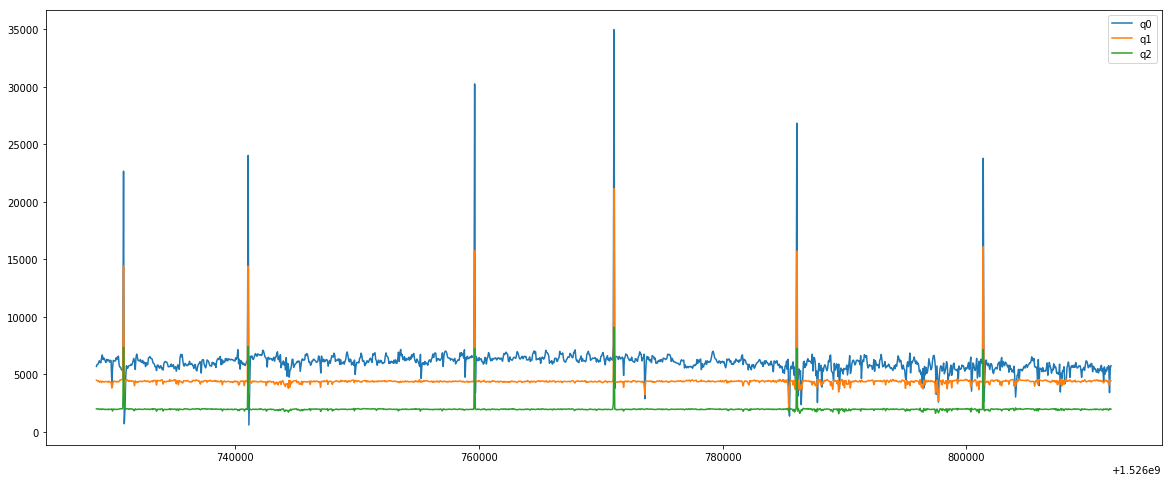
\includegraphics[width=\textwidth]{valid_cnt/valid_cnt}	
	
	\end{center}
	As convention, the blue, orange and green curves are 1-min expected messages number under QoS level respectively 0, 1 and 2.
\end{figure}

\begin{figure}
	\setlength{\tabcolsep}{0pt}
	\caption{topic: load/publish/dropped/1min}
	\label{f:valid_cnt_load_publish_dropped_1min}
	\begin{center}
	
		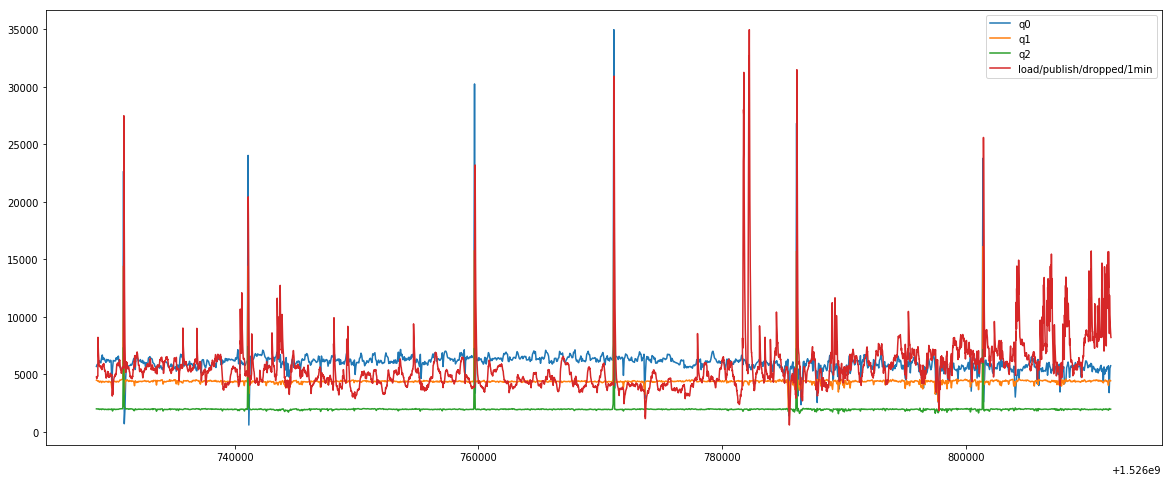
\includegraphics[width=\textwidth]{valid_cnt/valid_cnt-load_publish_dropped_1min}
	
	\end{center}
	It is observed that, surprisingly, the dropped messages largely correlates with the number of received expected messages, except for the fifth and jitters in the latter part (after the 3rd x-tick); it is reasonable because each peak is actually a publishing peak (in figure \ref{f:valid_cnt_load_messages_sent_1min}), when messages is dropped due to the jam. It is also noticed that curves for expected received messages has more jitters in the latter part as well, correlating with the dropped/1min curve.
\end{figure}

\begin{figure}
	\caption{topic: load/messages/sent/1min}
	\label{f:valid_cnt_load_messages_sent_1min}
	\begin{center}
		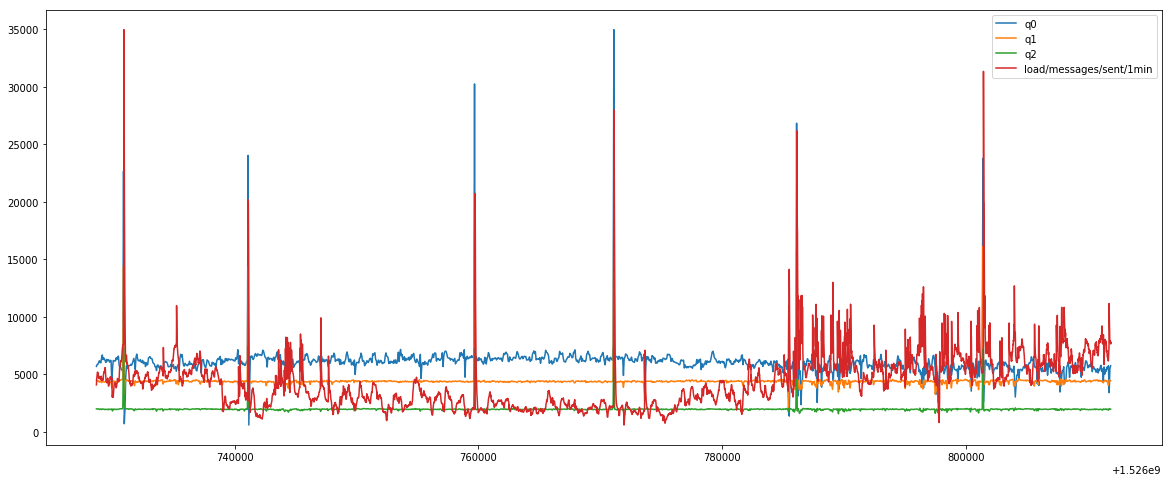
\includegraphics[width=\textwidth]{valid_cnt/valid_cnt-load_messages_sent_1min}
	\end{center}
	All the peak of 1-min expected messages number for each QoS nicely correlates with the sending peak from the SYS statics, which is expected because more it sends, more clients receive, and more chance for client to have an expected  sequential stream of received number.
\end{figure}

\begin{figure}
	\caption{topic: load/messages/received/1min}
	\label{f:valid_cnt_load_messages_received_1min}
	\begin{center}
		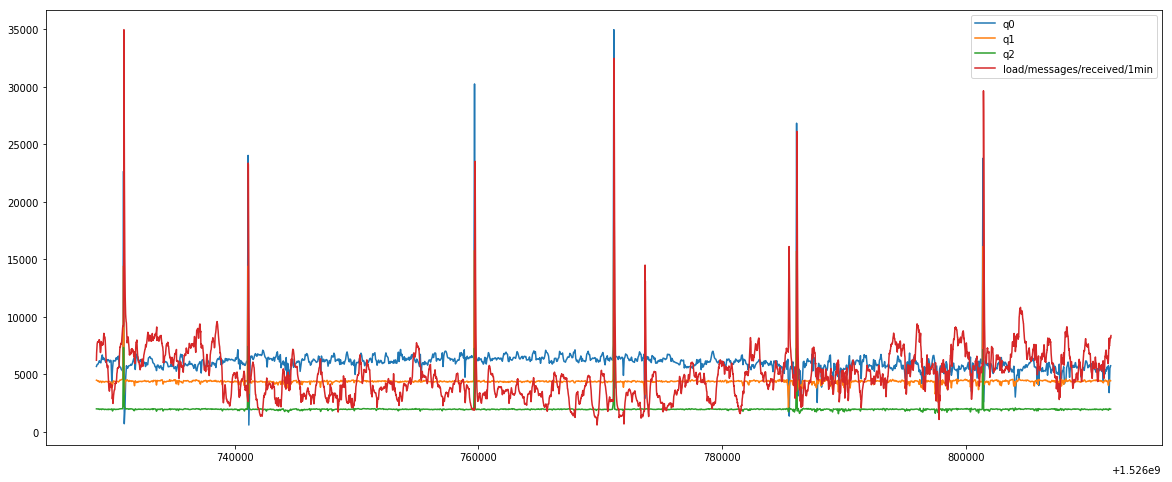
\includegraphics[width=\textwidth]{valid_cnt/valid_cnt-load_messages_received_1min}		
	\end{center}
	Again, all the peaks from SYS statics, except for some small peaks, correlates with curves for expected messages. This is expected because messages received by clients fundamentally come from the fast counter and broker needs to receives those numbers before passing them to clients.
\end{figure}

\begin{figure}
	\setlength{\tabcolsep}{0pt}
	\caption{topic: load/bytes/sent/1min}
	\label{f:valid_cnt_load_bytes_sent_1min}
	\begin{center}
		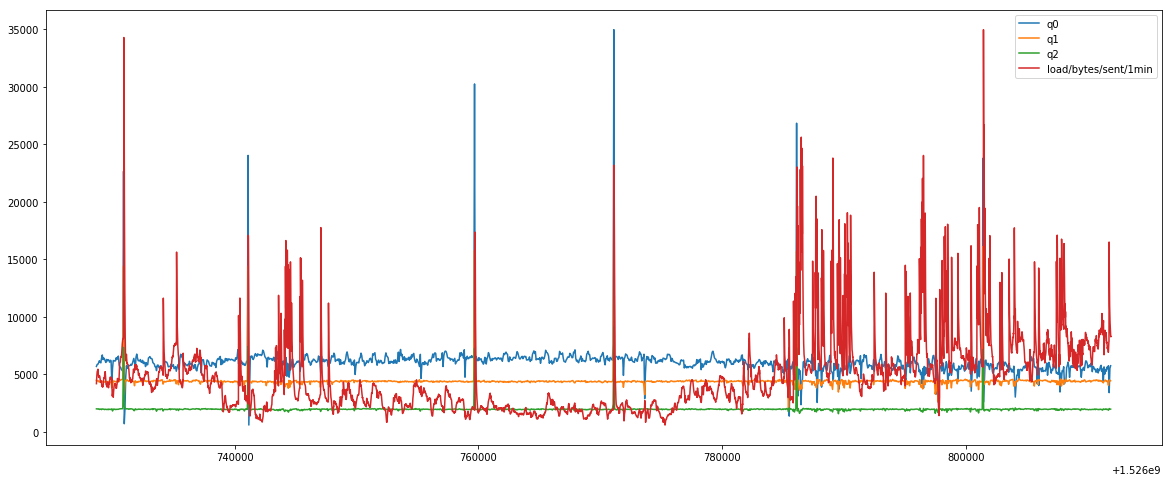
\includegraphics[width=\textwidth]{valid_cnt/valid_cnt-load_bytes_sent_1min}			
	\end{center}
	This is actually an interesting plot because it accounts for the size of each messages, where we can observe that on the left hand side around the first x-tick (740000) and after the third x-tick (780000), there are a number of small peaks of sending, denoting peaks of broker's work load for sending messages, which nicely correlates with those jitter-like peaks in previous figures (load/message/sent/1min: fig \ref{f:valid_cnt_load_messages_sent_1min}, load/publish/dropped/1min: fig \ref{f:valid_cnt_load_publish_dropped_1min}) 
\end{figure}

\begin{figure}
	\setlength{\tabcolsep}{0pt}
	\caption{topic: load/bytes/received/1min}
	\label{f:valid_cnt_load_bytes_received_1min}
	\begin{center}
		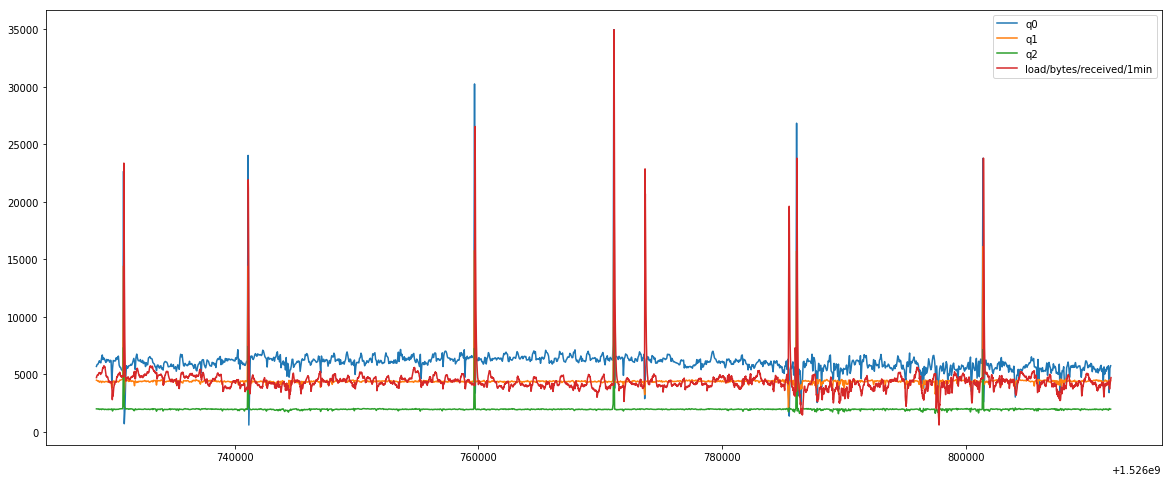
\includegraphics[width=\textwidth]{valid_cnt/valid_cnt-load_bytes_received_1min}	
	\end{center}
	It is however interesting that the messages received by the broker is not consistent with those outgoing peaks, especially those jitters. Then why would broker suddenly needs to send bigger and more messages?
\end{figure}

\begin{figure}
	\setlength{\tabcolsep}{0pt}
	\caption{topic: load/connections/1min}
	\label{f:valid_cnt_load_connections_1min}
	\begin{center}
		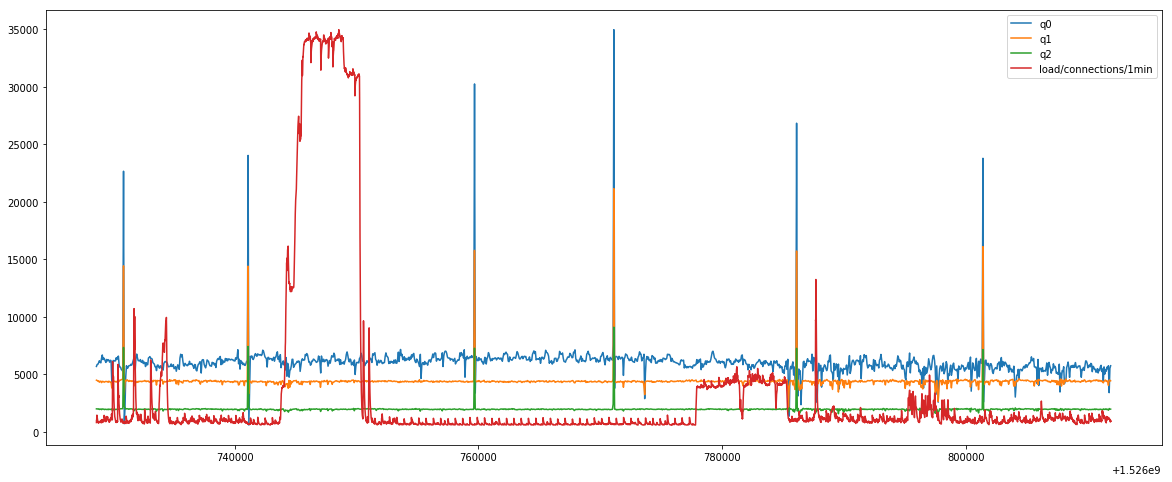
\includegraphics[width=\textwidth]{valid_cnt/valid_cnt-load_connections_1min}	
	\end{center}
	There is a burst of client requesting to connect but it seems to not correlate those jitters, indicating CONNECT packets itself would not have any instant impact.
\end{figure}

\begin{figure}
	\setlength{\tabcolsep}{0pt}
	\caption{topic: clients/connected}
	\label{f:valid_cnt_clients_connected}
	\begin{center}
		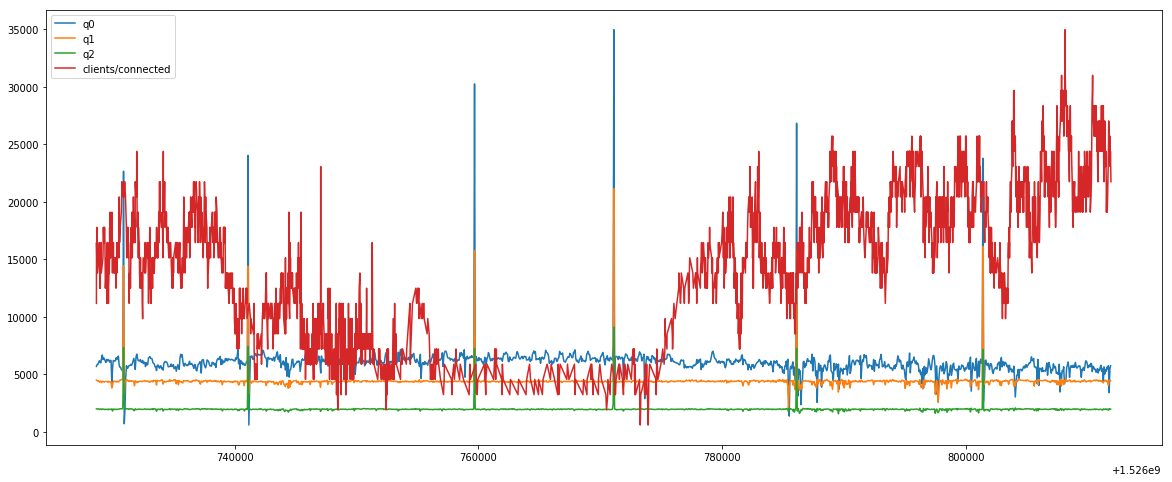
\includegraphics[width=\textwidth]{valid_cnt/valid_cnt-clients_connected}	
	\end{center}
	It is clear now in this figure that the number of active clients coorelates with those small peaks, or previously referred as jitters, where broker needs to send more messages and bytes out; and it is reasonable that broker sends more at when more clients connect and receive messages from broker, especially they may receive messages from other topic then topics subscribed by my clients, i.e. slow channel.
\end{figure}

\begin{figure}
	\setlength{\tabcolsep}{0pt}
	\caption{topic: heap/current}
	\label{f:valid_cnt_heap_current}
	\begin{center}
		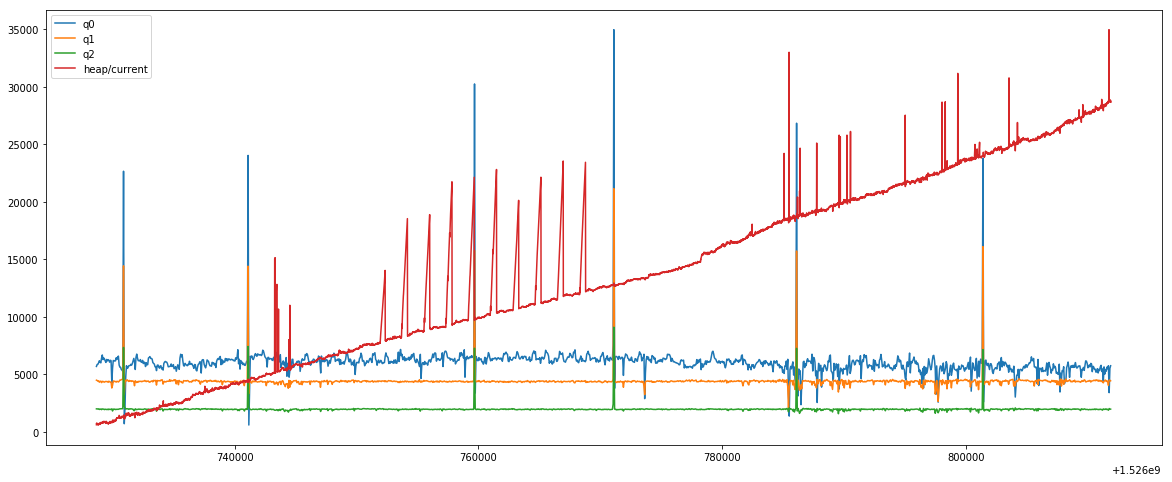
\includegraphics[width=\textwidth]{valid_cnt/valid_cnt-heap_current}	
	\end{center}
	It is expected to observe an increasing allocated memory on the broker because intuitively there will be more and more retained messages published from students to the broker; it actually nicely correlates with the number of retained messages in figure \ref{f:valid_cnt_retained} as expected. It is yet unexpected to see those small peaks along its increasing, denoting several memory burst and I could not find any coorelated curves with that in the given time of this assignment. It also seems to not correlate with the number of received expected messages.
\end{figure}

\begin{figure}
	\setlength{\tabcolsep}{0pt}
	\caption{topic: heap/maximum}
	\label{f:valid_cnt_heap_maximum}
	\begin{center}
		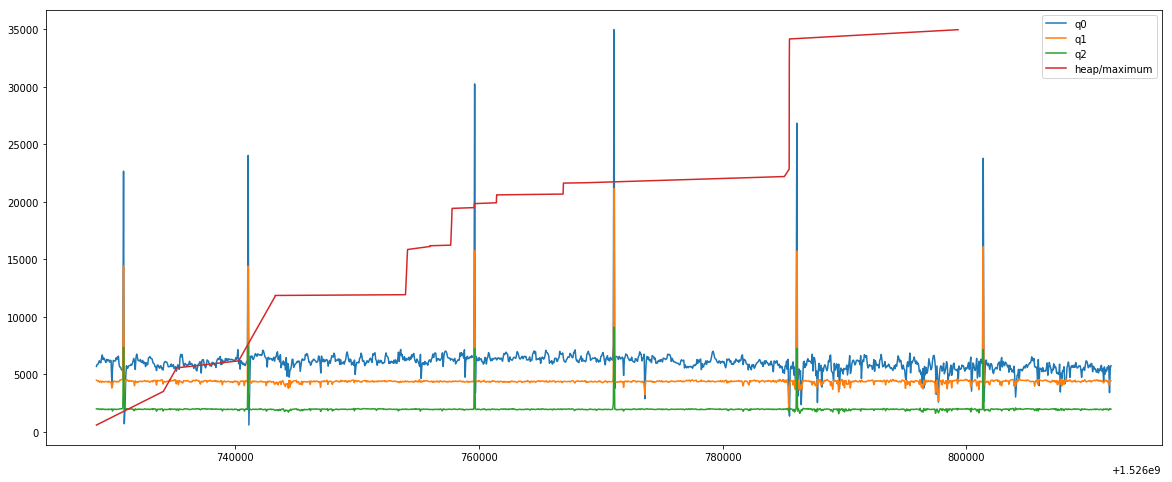
\includegraphics[width=\textwidth]{valid_cnt/valid_cnt-heap_maximum}
	\end{center}
	The maximum heap memory ever allocated is expected and correlates with the trends of the curve for current heap memory.
\end{figure}

\begin{figure}
	\setlength{\tabcolsep}{0pt}
	\caption{topic: messages/stored}
	\label{f:valid_cnt_messages_stored}
	\begin{center}
		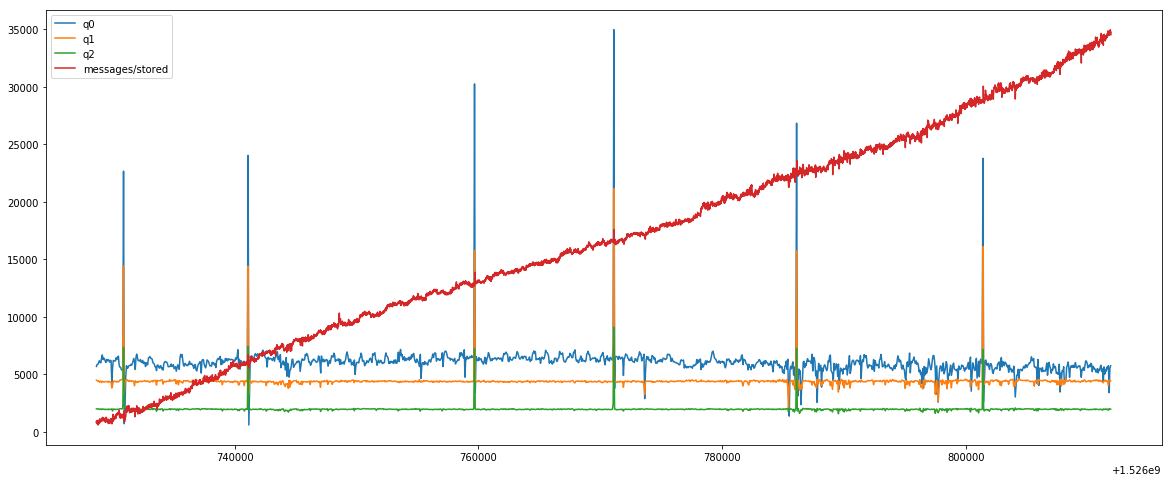
\includegraphics[width=\textwidth]{valid_cnt/valid_cnt-messages_stored}	
	\end{center}
	This is messages held in message store, including retained messages and in-queue messages waiting for delivery and being acknowledged under QoS level 1 and 2, which, as expected, correlates with retained messages and current heap memory, and seems to not correlate with the number of received expected messages.
\end{figure}
\begin{figure}
	\setlength{\tabcolsep}{0pt}
	\caption{topic: retained}
	\label{f:valid_cnt_retained}
	\begin{center}
		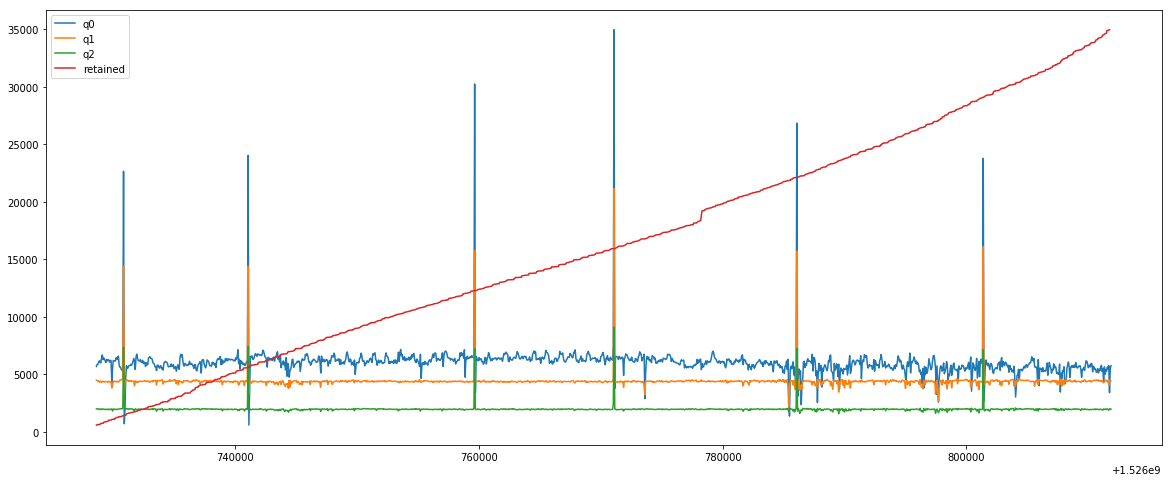
\includegraphics[width=\textwidth]{valid_cnt/valid_cnt-retained}	
	\end{center}
	The number of retained messages seems to be held in the heap memory and not correlates with or affects the expected messages received by clients or 
\end{figure}

\begin{figure}
	\setlength{\tabcolsep}{0pt}
	\caption{topic: publish/messages/dropped}
	\label{f:valid_cnt_publish_messages_dropped}
	\begin{center}
		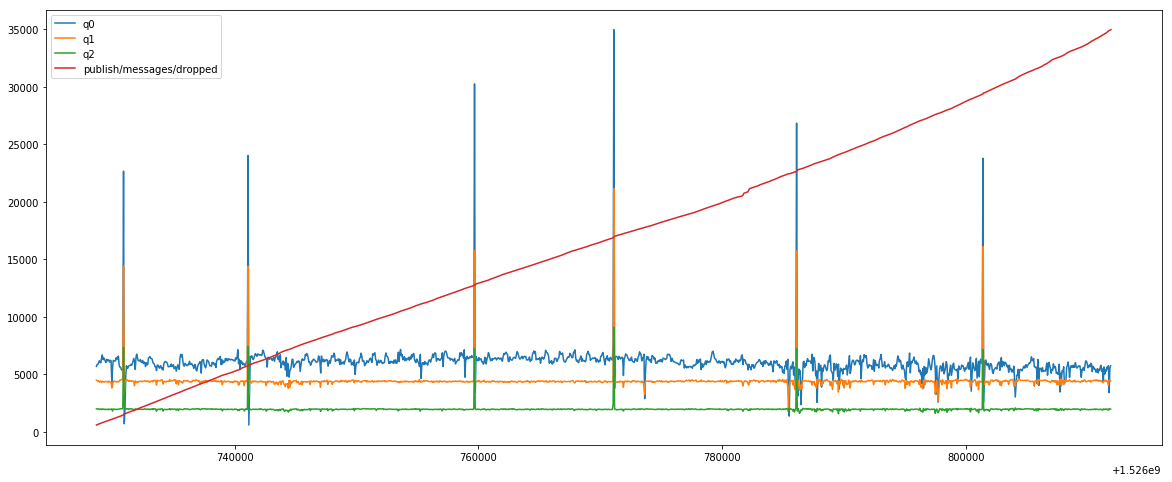
\includegraphics[width=\textwidth]{valid_cnt/valid_cnt-publish_messages_dropped}	
	\end{center}
	This is the total number of dropped messages due to inflight/queuing limits since the start, which is unexpected to not correlates with the number of clients' received expected messages, the received messages on the broker or the current heap memory allocated on the broker. The potential reason might be that the queues are allocated with a specialised memory instead of on the heap memory.
\end{figure}

\FloatBarrier
\subsubsection{10-min Loss Rate Correlating with \$SYS}
In this section, instead of using the total received expected message over 1 minute, we analyse the broker performance with loss rate, calculated with equation \ref{eq:loss_rate}. The out-of-order rate or duplicate rate are not analysed because they are too rare and thus do not have sufficient data.

It is surprising that during the period of this measurement, QoS level 0 is found to have 0 loss and QoS level 2 has a loss rate close to 0, compared to QoS level 1. Hence, the following graph will contain only curves from QoS level 1 and 2 on the background.

Similar to that in previous section \ref{s:1min_expected_msg}, the discussions are under each corresponding figure.

\FloatBarrier
\begin{figure}
	\setlength{\tabcolsep}{0pt}
	\caption{10-min loss rate under QoS 0,1,2}
	\label{f:loss_cnt}
	\begin{center}		
		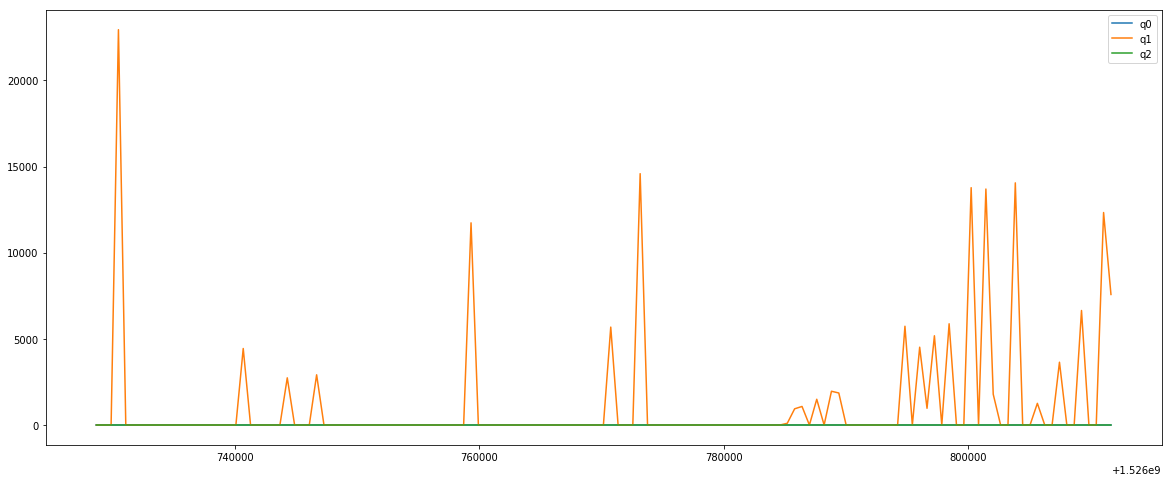
\includegraphics[width=\textwidth]{loss_cnt/loss} 
	\end{center}
	As convention, the blue, orange and green curves are 10-min expected messages number under QoS level respectively 0, 1 and 2. The loss rate of QoS level 0 is 0 and level 2 close to 0. Thus we only show the loss rate curve of QoS level 1 when comparing with SYS statics.
\end{figure}

\begin{figure}
	\setlength{\tabcolsep}{0pt}
	\caption{topic: load/publish/dropped/5min}
	\label{f:loss_cnt_load_publish_dropped_5min}
	\begin{center}
		
		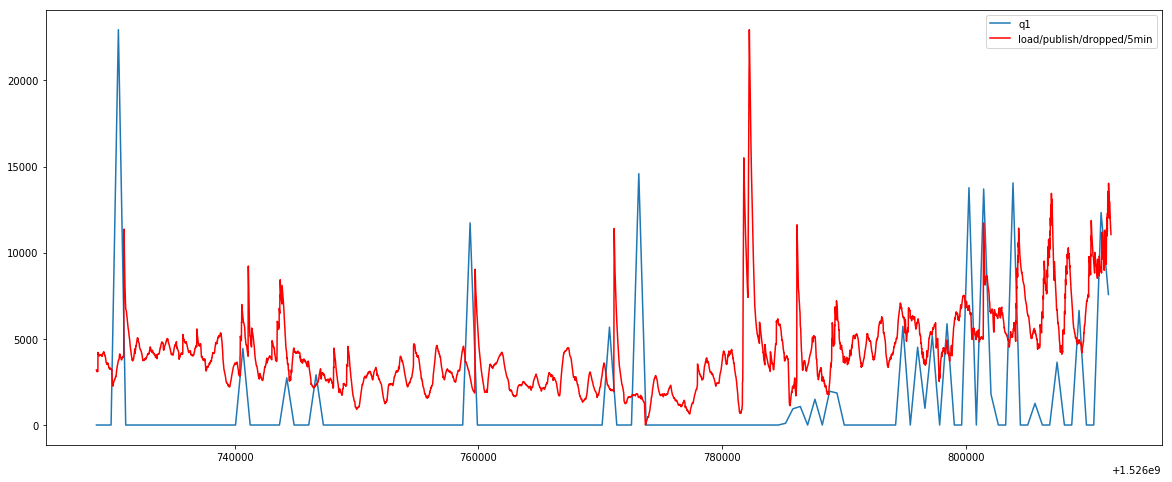
\includegraphics[width=\textwidth]{loss_cnt/loss-load_publish_dropped_5min}
		
	\end{center}
	It is observed that the dropped messages correlates with the loss rate as expected. It is interesting that the server becomes more and more stressed as the time goes, uncovered by the density of peaks in loss rate, which is denser in the latter part.
\end{figure}

\begin{figure}
	\caption{topic: load/messages/sent/5min}
	\label{f:loss_cnt_load_messages_sent_5min}
	\begin{center}
		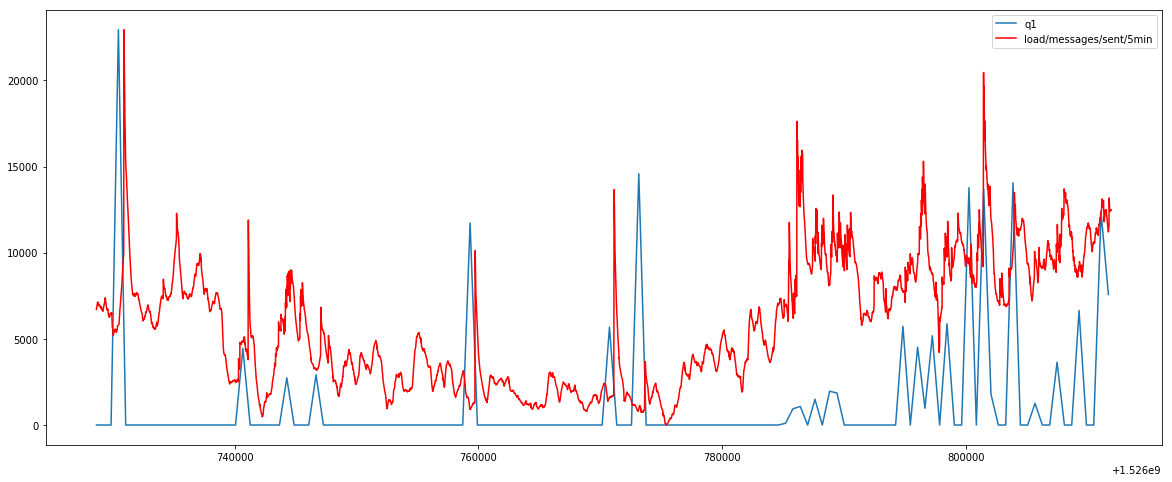
\includegraphics[width=\textwidth]{loss_cnt/loss-load_messages_sent_5min}
	\end{center}
	The loss rate curve barely correlates with the sending messages statics from broker. When broker needs to send more messages at latter part, the loss rate curve has more peaks. Or, in the other word, the more it needs to send, the more likely clients have lost messages.
\end{figure}

\begin{figure}
	\caption{topic: load/messages/received/5min}
	\label{f:loss_cnt_load_messages_received_5min}
	\begin{center}
		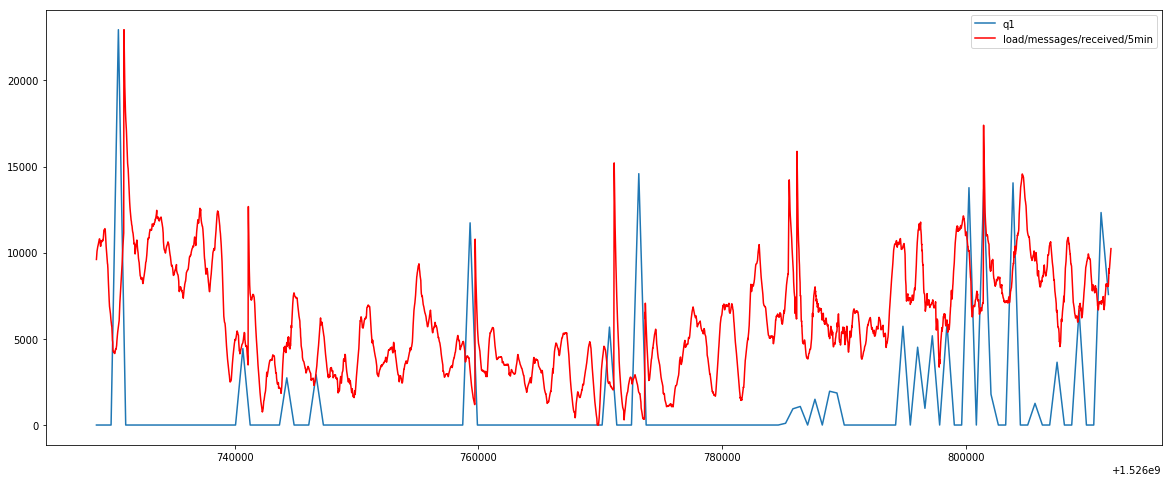
\includegraphics[width=\textwidth]{loss_cnt/loss-load_messages_received_5min}   
	\end{center}
	The curve for received messages at broker seems not to correlate with the loss rate curve, which is expected because the received messages are largely from counter on a relatively steady pace.
\end{figure}

\begin{figure}
	\setlength{\tabcolsep}{0pt}
	\caption{topic: load/bytes/sent/5min}
	\label{f:loss_cnt_load_bytes_sent_5min}
	\begin{center}
		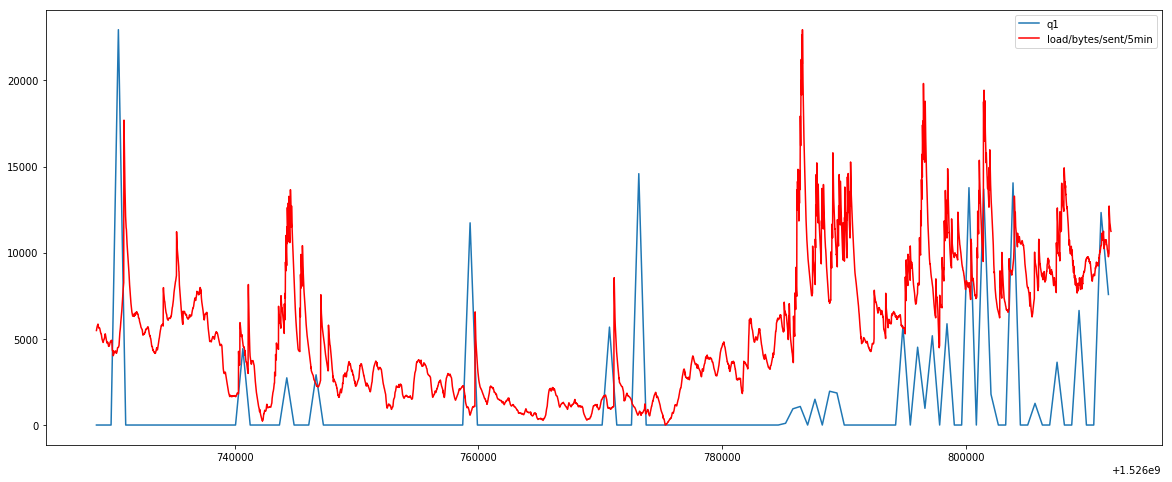
\includegraphics[width=\textwidth]{loss_cnt/loss-load_bytes_sent_5min}      
	\end{center}
	Apart from the correlation within SYS statics, (discussed in figure \ref{f:valid_cnt_load_bytes_sent_1min}), it also largely correlate with the loss rate curve, which is reasonable as more burden on the broker's task of sending will result in more loss rate.
\end{figure}

\begin{figure}
	\setlength{\tabcolsep}{0pt}
	\caption{topic: load/bytes/received/5min}
	\label{f:loss_cnt_load_bytes_received_5min}
	\begin{center}
		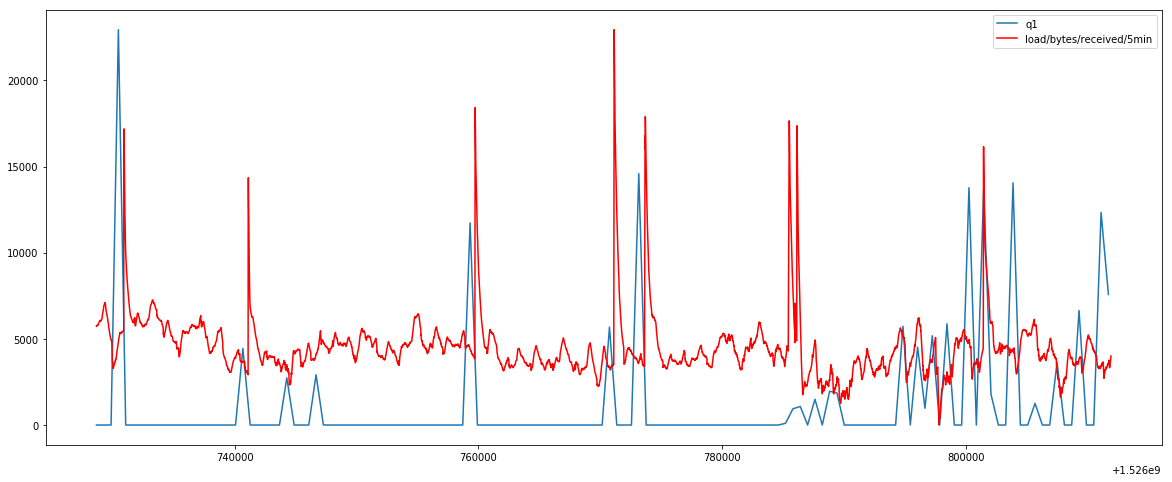
\includegraphics[width=\textwidth]{loss_cnt/loss-load_bytes_received_5min}  
	\end{center}
	This figure becomes interesting because curve for received bytes starts from largely correlating with loss rate curve and then ends up with not quite correlated. Such phenomenon is understandable because the received bytes over 5 minutes should reveal the burden of the broker's task of handling messages and denominates the loss rate, until another factor, the number of client, becomes large enough to affect the loss rate in the latter of this record. 
\end{figure}

\begin{figure}
	\setlength{\tabcolsep}{0pt}
	\caption{topic: load/connections/5min}
	\label{f:loss_cnt_load_connections_5min}
	\begin{center}
		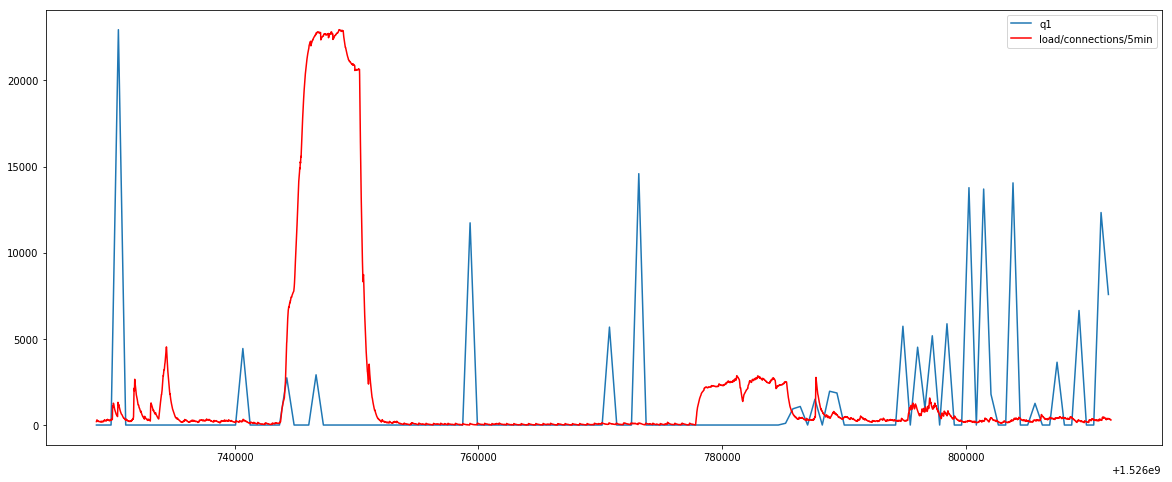
\includegraphics[width=\textwidth]{loss_cnt/loss-load_connections_5min} 
	\end{center}
	Similar to previous section, the CONNECT packets do not directly impact or correlate with the clients' statics, loss rate in this case.
\end{figure}

\begin{figure}
	\setlength{\tabcolsep}{0pt}
	\caption{topic: clients/connected}
	\label{f:loss_cnt_clients_connected}
	\begin{center}
		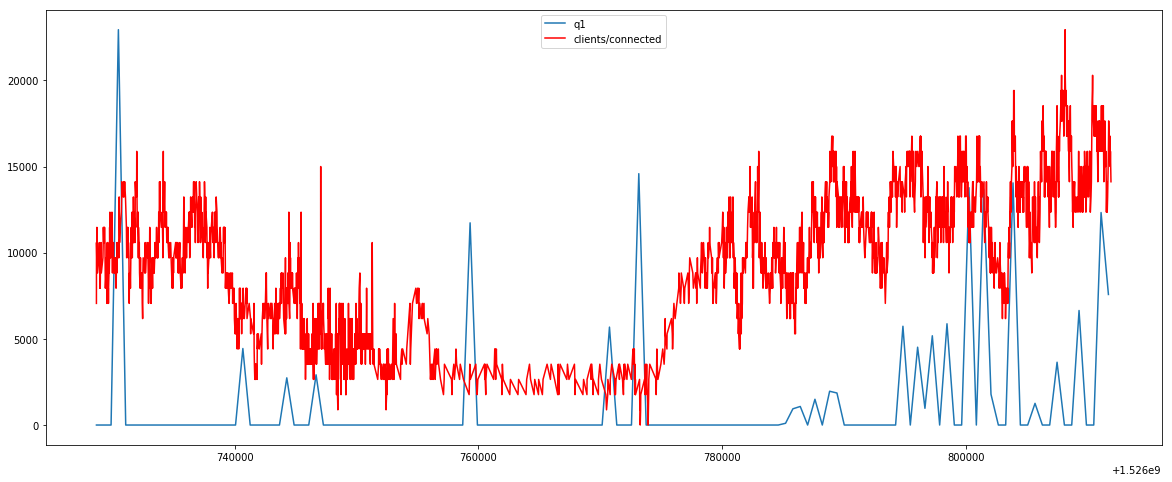
\includegraphics[width=\textwidth]{loss_cnt/loss-clients_connected} 
	\end{center}
	As discussed in previous section \ref{s:1min_expected_msg}, the active clients are a key role in influencing broker's performance. We observe and expect to observe that as more clients connected to the broker in the latter part, more peaks in loss rate curve show up.
\end{figure}

\begin{figure}
	\setlength{\tabcolsep}{0pt}
	\caption{topic: heap/current}
	\label{f:loss_cnt_heap_current}
	\begin{center}
		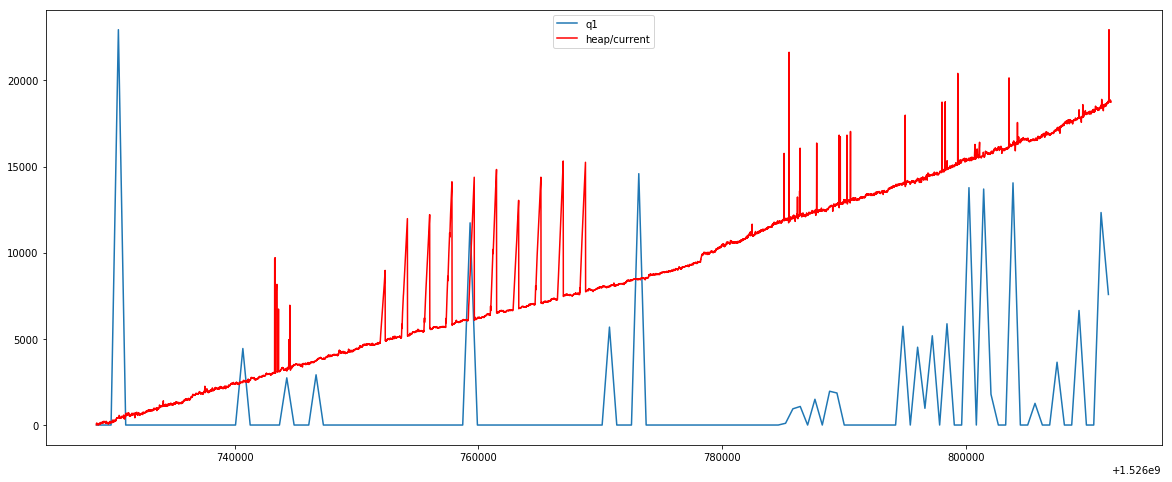
\includegraphics[width=\textwidth]{loss_cnt/loss-heap_current}  
	\end{center}
	As discussed in previous section \ref{s:1min_expected_msg}, the current heap memory correlates with the number of both retained and stored messages in broker and also the maximum heap memory used. Yet it is not considered correlated with clients' statics, loss rate in this case. Hence, for simplicity, the analysis for correlation between loss rate curve and curves for topics of heap/maximum, messages/stored and retained are not shown here; and the result is the same as the analysis between curves for expected messages and those topics.
\end{figure}

\FloatBarrier
\section{Analysis and Correlation between Students' Report}


\section{Real-World Analysis}
Consider the broader end-to-end network environment, in a situation with many thousands of
sensors publishing regularly to some large number of subscribers. Explain in your report

\subsection{Performance Challenges}

\subsubsection{End-network: Sources and Clients}
The challenge at source would be dependent on actual task. In the case of master-slave model, where the source are only responsible for publishing messages and performs only one-way communication, the challenge for CPU and memory of source are small, because it only needs to support its own use. It is yet challenging for sources to dynamically recognise and adapt to the clients requirement or constraint. Such challenge will transit to the clients, whose CPU and memory should be able to catch up with the sources and cope with potential incoming messages burst. 

While in the case where two-way communication between clients and sources exists, the challenge of adapting to each other are reduced; nonetheless the sources need to cope with different requirement from various clients, which can forms a challenge for the sources' ability of offering the services in different forms or under different conditions in parallel.

The network challenge here is the well-known last-mile challenge. The last-mile network can be under different situation and exposed to various noise, which potentially requires the sources and clients to be aware of such condition if used in the IoT / IoE architecture.

\subsection{Intermediate: Broker}

The broker in MQTT becomes a bottleneck, also known as single failure point, of the overall performance. It is because all the messages need to first collected into the broker and then distributed to the corresponding clients in their preferred way.

As also mentioned in challenges for sources, the broker needs to have enough ability to provide three different services. It also becomes a huge challenge for CPU and memory on the broker because even if a few sources happen to have a output burst it will add up and potentially arrives together on the broker. 

The memory consumption is another challenge because not only messages on the fly needs enough space for itself or acknowledgement, but also retained messages are likely to constantly take up spaces on the broker and might cause the service to degrade when free memory is low.

The network at the broker is crucial, because the network is not only more likely to be jammed because of output burst from the sources, but also can heavily influence the efficiency of broker's sending out the messages in queue. If the outgoing network is always not as efficient as the incoming network, the broker's limited memory is going to run out eventually.

\subsection{Different QoS Levels for Challenges}

To ease the pain of sources not knowing the performance limit on clients, QoS level 1 or 2 can be helpful, depending on if the occurrence of message matters, as discussed under figure \ref{fig:handshake_snap_shot}. Because in QoS level 1 or 2, broker handles the acknowledgement of the messages on behalf of the sender.

However, QoS level 1 or 2 can brings server burden onto the broker, because messages need to take up the resources on broker both longer and more. Such burden may add up to a point where broker needs to break the specification in protocol due to physical limits.

To prevent the bottleneck from limiting the overall performance, it is suggested to use QoS level 0, where sources and clients may need to handle the acknowledgement and adaptation by themselves. In return, the broker is able to have less CPU and memory burden. Nonetheless, it is worth noting that the network burden may not be reduced or may even be enhanced if clients and sources decide to handle acknowledgement by themselves. Overall, QoS level 0 can reduce the broker's stress.

\subsection{Comparison with Measurement}

Interestingly, regarding averaged 10-min loss rate, the QoS level 0 performs the best, with 0.0 10-min loss rate; the QoS level 2 the second, with 1.4 10-min loss rate; and the QoS level 1 the worst, with 5259 10-min loss rate. While regarding the number of received expected messages, QoS level 0 , 1 and 2 reaches an average of 5842, 4620 and 2203 over 1-min interval during the measurement. The measurement here are all from 2018-05-19 21:17:50 to 2018-05-20 20:22:14, measured in parallel.

It is expected that QoS level 0 actually performs the best because that part of broker is able to cater everybody on a nearly constant pace as the incoming speed is almost constant and the number of clients are roughly 500 according to the SYS statics. Given a relatively stable network environment in ANU (thanks to network team), the performance is close to perfect as expected. Hence, QoS level 0 might be able to send at a comparable speed with the speed for incoming messages from counter; and thus achieving a 0.0 loss rate and the most messages received on average.

It is yet unexpected that the QoS level 2 would outperforms the level 1, regarding the loss rate. The proposed reason is that the sources publish message in QoS level 1 and may jam the corresponding memory more often because it does not care the duplication. In other word, QoS level 2 is able to stop for a little while because of its 4-way handshake, whereas in QoS level 1 there is no gap between the publish of two numbers, causing the broker to be under a relatively high burden in terms of available slots in messages queue.

The above proposed reason is also consistent with the total expected messages each QoS level receives. That is, the QoS level 1 receives much more than that of QoS level 2 in 1-min interval and thus operating in high speed and stressing the broker out more often and QoS level 2 receives on average only a half of the QoS level 1 over the 1-min interval.

\end{document}